\section{Asymmetric Diagnostics}\label{app:mode-comparison}

Source-weighted and target-weighted modes diagnose which side carries the mismatch. Figure~\ref{fig:mode-comparison} isolates contamination on the source side, target side, or both. Source-weighted corrects source-only mismatch; target-weighted corrects target-only mismatch. Only the doubly weighted test remains calibrated under two-sided mismatch. When mismatch is known to be one-sided, the asymmetric modes offer lower-variance alternatives.

The overlap-vs-stabilized contrast is sharpest here. Overlap weights assign the same weight function $e(1-e)$ to both groups, so they cannot distinguish which side carries the non-comparable mass---they over-reject under two-sided mismatch at the same rate as the unweighted test. Crump trimming drops extreme-propensity observations symmetrically and therefore also fails under two-sided mismatch. The asymmetric RIW corrections---forward for source, inverse for target---are the only weighting scheme that adapts the correction to each group's density structure independently.

\begin{figure}[t]
	\centering
	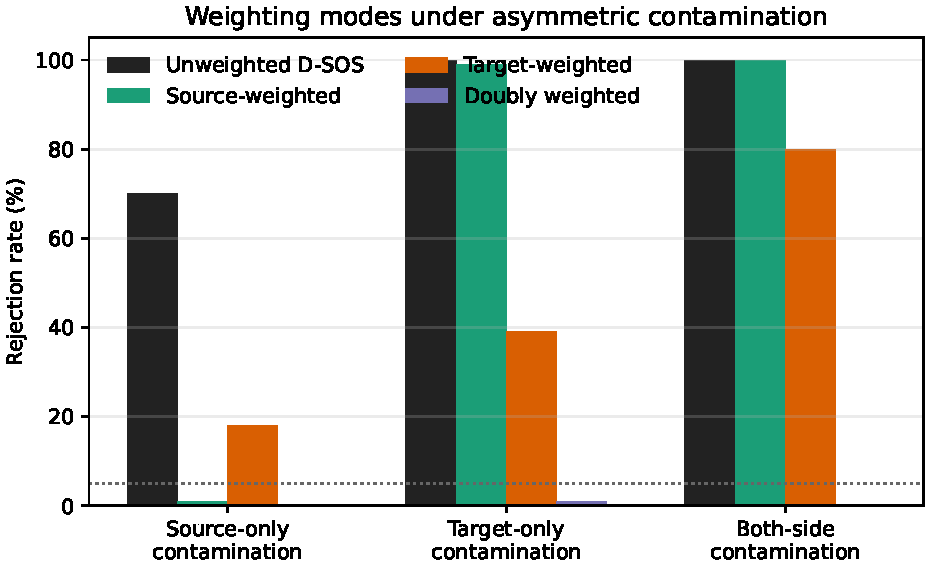
\includegraphics[width=0.95\linewidth]{figures/mode_comparison_plot.pdf}
	\caption{Asymmetric-diagnostic study. Contamination pattern (source-only, target-only, or two-sided) versus rejection rate. The dotted line marks the $5\%$ nominal level. Source-weighted and target-weighted diagnostics help only for one-sided contamination. The doubly weighted test remains calibrated when both sides contain irrelevant weak-overlap mass.}
	\label{fig:mode-comparison}
\end{figure}

\section{Second Synthetic Data-Generating Process}
\label{app:second-dgp}

The main text uses a univariate Gaussian overlap model. This appendix reports a second synthetic DGP with two-dimensional features and a linear score function. Source features are drawn from $\mathcal{N}(0, I_2)$. Target features are a mixture: $(1-\delta)$ fraction from $\mathcal{N}(0, I_2)$ and $\delta$ fraction from $\mathcal{N}((3,0), 0.5 \cdot I_2)$, where $\delta$ is the overlap-severity parameter. The severity score is $S = 0.5X_1 - 0.3X_2 + \epsilon$ with $\epsilon \sim \mathcal{N}(0, 0.5)$ for both groups, and harmful shift adds an intercept term to target scores on the common support. The domain classifier uses the first feature dimension only.

Figure~\ref{fig:second-dgp-calibration} confirms the calibration pattern: the doubly weighted test stays near nominal while unweighted testing over-rejects as overlap weakens. Figure~\ref{fig:second-dgp-power} shows power under harmful shift on the common support: the doubly weighted test responds to genuine harm while remaining calibrated at zero effect.

\begin{figure}[t]
	\centering
	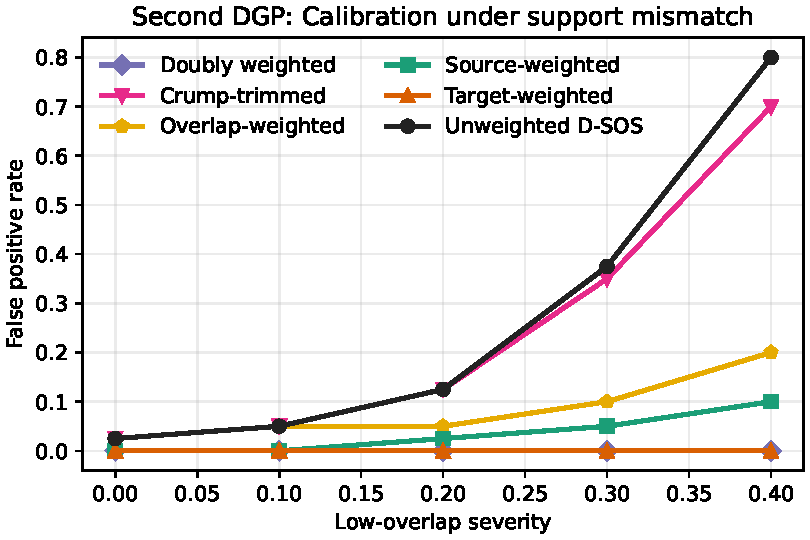
\includegraphics[width=0.95\linewidth]{figures/second_dgp_calibration_plot.pdf}
	\caption{Calibration under the second DGP. The doubly weighted test preserves calibration while unweighted and one-sided modes over-reject.}
	\label{fig:second-dgp-calibration}
\end{figure}

\begin{figure}[t]
	\centering
	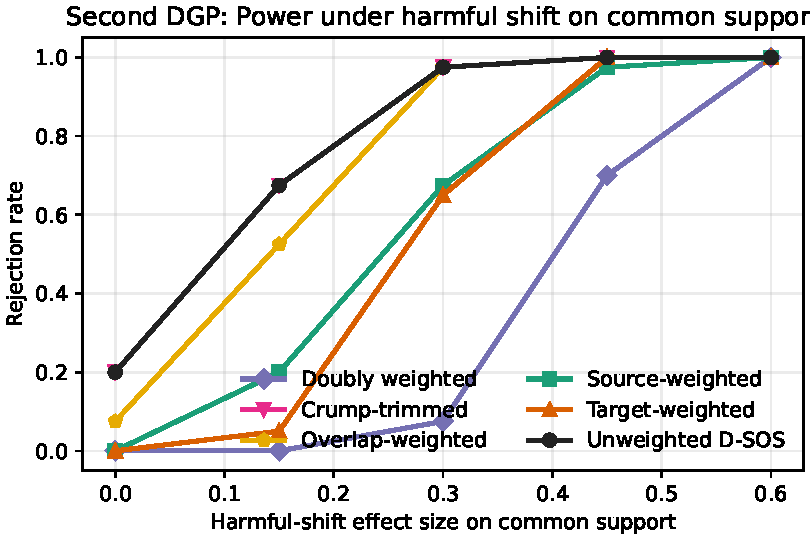
\includegraphics[width=0.95\linewidth]{figures/second_dgp_power_plot.pdf}
	\caption{Power under the second DGP. The doubly weighted test detects harmful shift on the common support while remaining specific at zero effect.}
	\label{fig:second-dgp-power}
\end{figure}

\section{Domain Classifier Sensitivity}
\label{app:domain-clf-sensitivity}

The main text uses logistic regression as the domain classifier. This appendix reports calibration under three classifier families: logistic regression, random forest ($100$ trees, max depth $5$), and histogram gradient boosting ($100$ iterations). The experiment replicates the calibration setup from the main text for each classifier.

Table~\ref{tab:domain-clf-sensitivity} reports the rejection rate of the doubly weighted test at each severity level. All three classifiers produce similar calibration: the doubly weighted test stays near the nominal $5\%$ level across the severity grid. The random forest and HistGBM produce more concentrated weights (lower ESS) because their flexible decision boundaries separate source and target more sharply, but this does not inflate false alarms.

\paragraph{Real-data classifier and split robustness.} The synthetic study isolates classifier choice; for the revision the HELOC checks will be repeated with an alternative domain classifier (random forest) and a perturbed split (ExternalRiskEstimate $>60$) to confirm the reported ESS and $p$-value regime. Committed \texttt{results/} and \texttt{figures/} were regenerated at the current protocol (9,999 permutation resamples, ten-fold domain-classifier CV); metadata hashes match the current tree (see Reproducibility Plan).

\begin{table}[t]
	\centering
	\caption{Doubly weighted rejection rate by domain classifier and severity (40 repeats, $\lambda = 0.5$).}
	\label{tab:domain-clf-sensitivity}
	\footnotesize
	\begin{tabular}{l c c c}
		\toprule
		Severity & Logistic & Random Forest & HistGBM \\
		\midrule
		0.0 & 0.00 & 0.00 & 0.00 \\
		0.1 & 0.00 & 0.00 & 0.00 \\
		0.2 & 0.00 & 0.00 & 0.00 \\
		0.3 & 0.00 & 0.03 & 0.00 \\
		0.4 & 0.00 & 0.00 & 0.03 \\
		\bottomrule
	\end{tabular}
\end{table}

\section{NSW Employment Experiment (Raw Outcome Score)}\label{app:nsw}

The National Supported Work (NSW) program~\cite{LaLonde_1986} contrasts experimental treated participants with an observational comparison group. We use the Dehejia--Wahba screened CPS comparison sample ($n=429$; evaluation $n=85$ after the source holdout) as source and the NSW treated group ($n=185$) as target, with post-program earnings in dollars as a continuous, higher-is-better severity score and no model-derived score (9,999 permutation resamples). Populations differ systematically in education, prior earnings, and demographics, creating feature overlap that mirrors weak-overlap settings from the synthetic experiments (doubly weighted ESS: $24$ of $85$ source, $57$ of $185$ target evaluation observations). The test does not reject under any mode (unweighted $p=0.131$, doubly weighted $p=0.508$; Crump-trimmed $p=0.660$, overlap-weighted $p=0.604$). Mean earnings are higher in the source ($\$7{,}832$) than in the target ($\$6{,}349$), yet no test flags the difference---contamination can mask harm as readily as it invents it. About a quarter of each group reports zero earnings, so ties are present but mild; the outcome is continuous dollars rather than a binarized threshold. The non-rejection should be read alongside the HELOC illustration in the introduction that contamination can both invent harm and hide it.
